\subsection{Driver Responses to Air Pollution Exposure}
This section explores how drivers responded to the observed air pollution patterns, combining quantitative findings with qualitative insights from interviews and driver archetypes (``Income-Driven'' and ``Health-Conscious'').
While quantitative analysis reveals complex exposure patterns varying temporally (\autoref{fig:daily-pollution-per-driver}, \autoref{fig:hourly-work-aqi}) and spatially (\autoref{fig:subdistrict-aqi}) across individuals and cities,
driver responses show limited adaptation, dictated primarily by economic needs and the perceived unavoidability of pollution.

\subsubsection{Prioritizing Income Amidst Pervasive Pollution}
Our analysis reveals no correlation between drivers' daily work hours and concurrent average PM2.5 levels (\autoref{fig:work-hours-vs-aqi-per-rider}), indicating a lack of temporal work adjustments in response to pollution fluctuations.
This aligns with qualitative interviews where drivers frequently expressed perceiving pollution exposure as an unavoidable occupational hazard rather than a modifiable risk.
Many prioritized immediate income over avoiding polluted times, echoing sentiments like,

\begin{quoteb}
    ``I just go where the application tells me to go, ..., the (air) pollution is everywhere anyway.'' (BKK1)
\end{quoteb}

\begin{quoteb}
    ``When I see that the area gets smoggier, I often thought about driving out to the suburban area. But that means I'll have to drive an empty car out.'' (BKK5)
\end{quoteb}

This ``Income-Driven'' approach was common.
Driver BKK1 (46, Male), targeting 2,000-2,500 baht daily through long hours (4 AM-9 PM), exemplified this.
Despite experiencing symptoms like runny noses and eye irritation and becoming aware of pollution levels via our map visualization after joining the study, his driving patterns remained unchanged.
He explained his reliance on masks and persistence:

\begin{quoteb}
    ``I can feel my body gets weaker (the more I drive); I always wear masks. ... If Google Maps tells us to go, I go. Wherever it is, I just have to push through.'' (BKK1)
\end{quoteb}

He further emphasized the lack of choice dictated by the platform and financial needs:

\begin{quoteb}
    ``I will not be able to be selective about routes; I go wherever the application assigns me to go, no matter of how far or how polluted the area may be.'' (BKK1)
\end{quoteb}



The dominant narrative remains that immediate economic needs override pollution avoidance strategies concerning work timing.

\subsubsection{Limited Mitigation}
While prioritizing income was dominant, some drivers, exemplified by the ``Health-Conscious'' driver BKK3, attempted mitigation strategies within existing constraints.
BKK3 (54, Female) actively incorporated heightened air pollution awareness into driving decisions after using the sensor helmet and map visualization.
She observed pollution spikes when riding behind buses,
\begin{quoteb}
    ``When I follow big buses, the graph just shoots up immediately.'' (BKK3)
\end{quoteb}

and gained insight into hazardous AQI levels (80-100 \textmu{}g/m$^3$) even on seemingly clear days. This awareness prompted actions like avoiding main roads for side streets, despite potentially longer distances,
\begin{quoteb}
    ``Main roads have more dusts (air pollutants), it’s better to go through small alleys.'' (BKK3)
\end{quoteb}

and selectively accepting rides or disabling auto-matching nearby to reduce prolonged exposure, particularly when heading home.


However, despite finding the real-time, localized AQI data useful, financial needs prevailed:

\begin{quoteb}
    ``We took this job for the money. We just have to live with it.'' (BKK3)
\end{quoteb}

BKK3's experience illustrates the tension between health awareness and economic necessity.
While information tools provide valuable insights, platform constraints significantly limit drivers' ability to act on this information without sacrificing income.

In this study, we do not observe a correlation between drivers' mitigation behaviors and their age or gender.

\subsubsection{Increased Awareness and Community Engagement}
Participation in the study and access to the map visualization significantly increased drivers' awareness and spurred public engagement.
Most participants reported frequently checking the visualization, particularly on high-pollution days.
This led to discussions about air quality with friends and passengers; for instance, CMI4 advised others on mask use, while BKK4 shared real-time data from the visualization with passengers during rides in poor conditions.
The visualization thus served both as a personal reference tool and a catalyst for community awareness.

Driver CMI1 exemplified proactive community engagement.
He monitored morning pollution levels and actively shared warnings in the Chiang Mai rideshare driver community (>5,000 members) when conditions were hazardous:

\begin{quoteb}
 ``I often take a screenshot (of the map visualization) when the air pollution levels turn red (hazardous) and share it in the group, warning everyone to be extra careful since the pollution got worsen that day.'' (CMI1)
\end{quoteb}

This demonstrates how access to real-time, localized data empowered drivers beyond personal monitoring.
It fostered collective awareness and turned some participants, like CMI1, into informal educators and active contributors to environmental health knowledge sharing within their community, moving beyond passive data reception.

\begin{figure*}
    \centering
    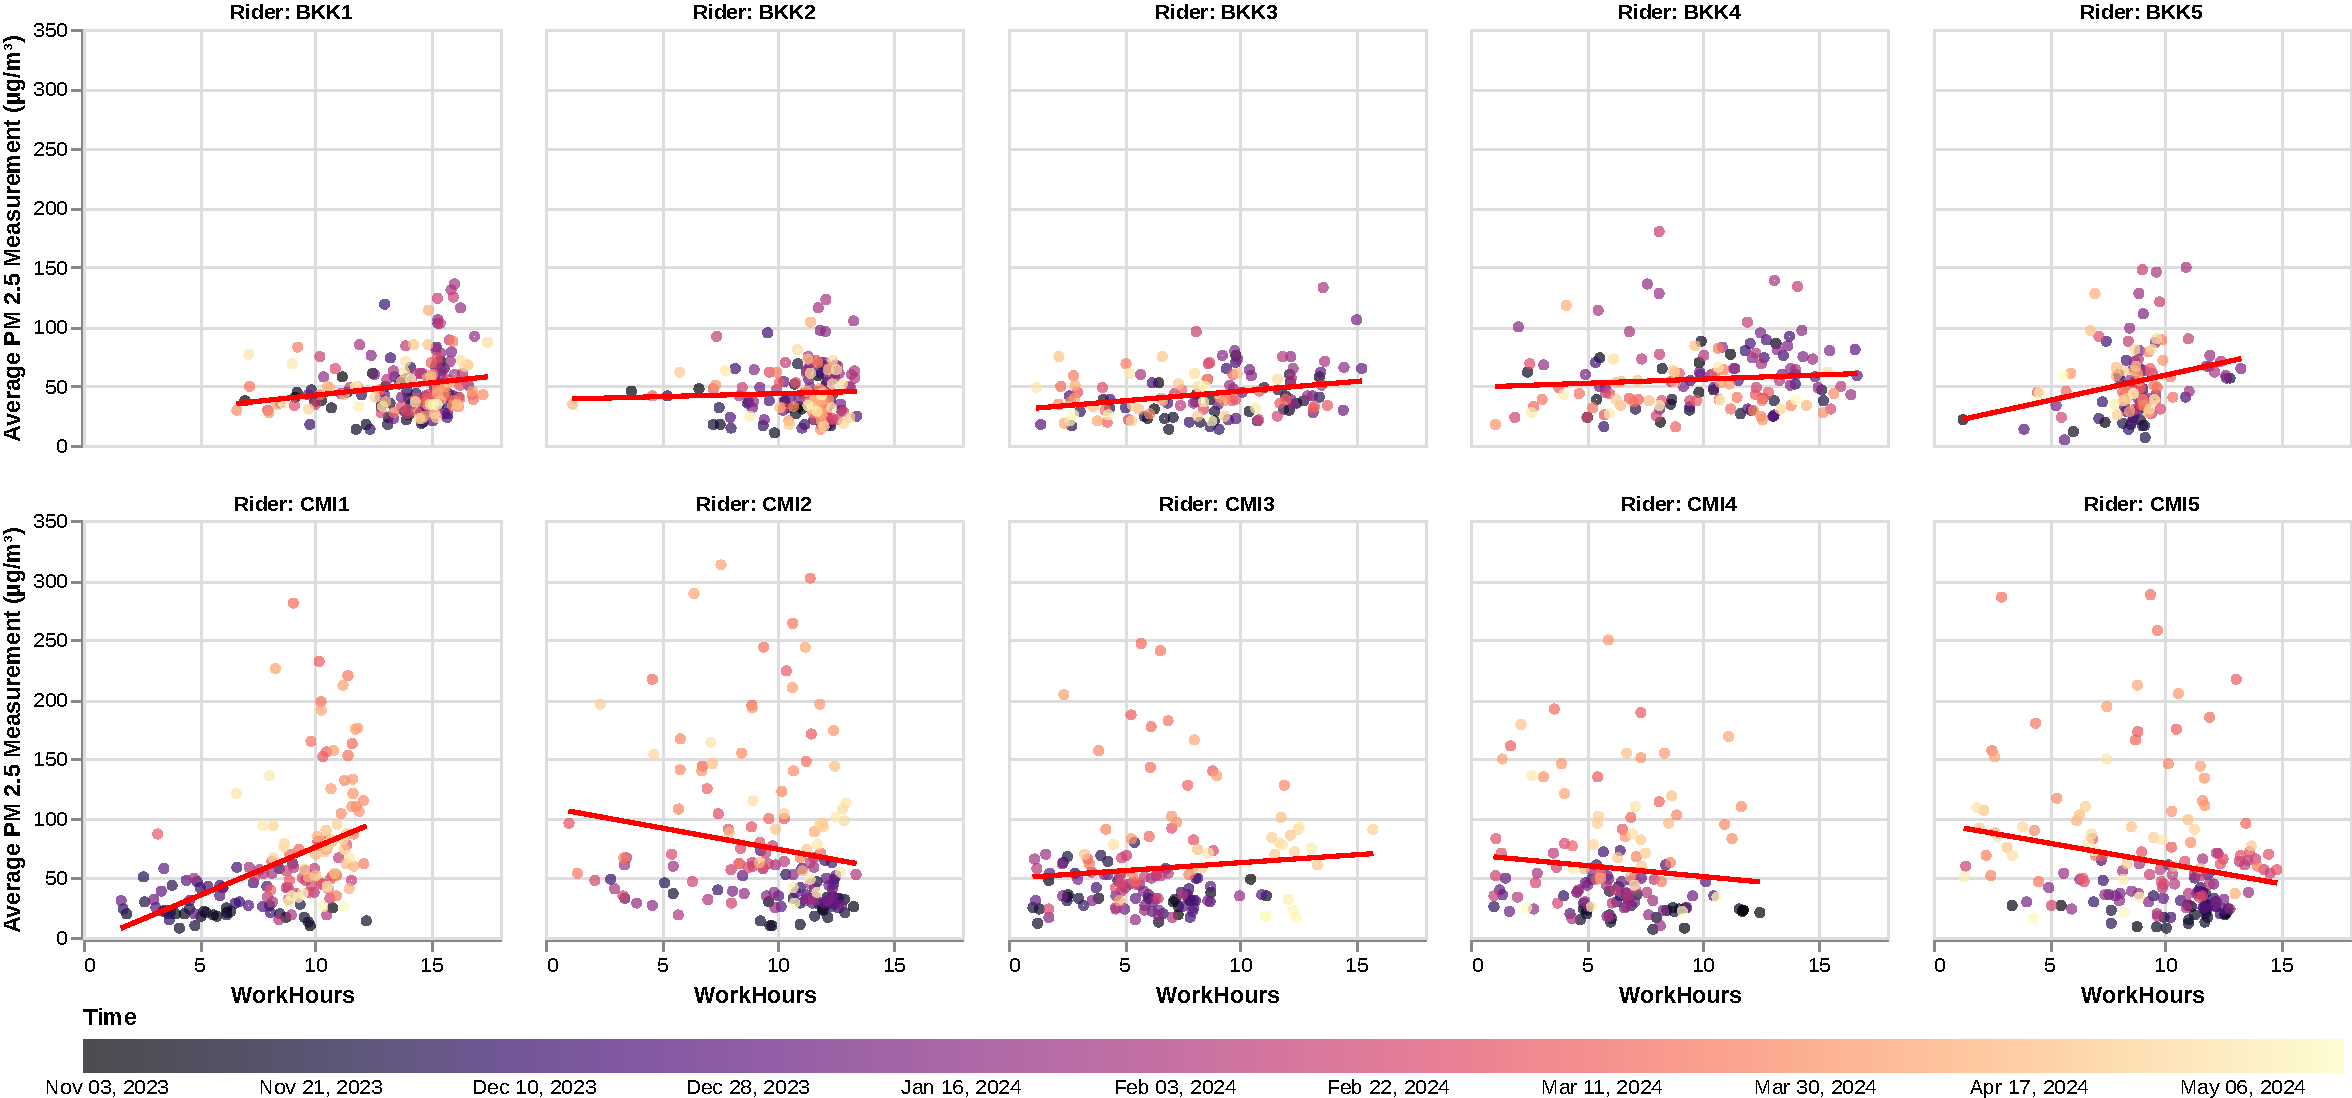
\includegraphics[width=\textwidth]{figures/work-hours-vs-aqi-per-rider-regression.pdf}
    \caption{Correlation of daily work hours and air pollution measurement for each driver, averaged through each week, with regression lines.
    }
    \Description{}
    \label{fig:work-hours-vs-aqi-per-rider}
\end{figure*}

Overall, while access to air quality information increased awareness and even spurred community engagement, the demanding nature of gig work and the perceived ubiquity of pollution limit drivers' capacity to translate this awareness into significant behavioral changes, particularly regarding work schedules.
Financial imperatives largely override health considerations, highlighting the need for systemic interventions beyond individual information provision to effectively reduce exposure, such as low-emission zones or integrating real-time AQ data into traffic management.
